% RECOMMENDED %%%%%%%%%%%%%%%%%%%%%%%%%%%%%%%%%%%%%%%%%%%%%%%%%%%
\documentclass[graybox]{svmult}

% choose options for [] as required from the list
% in the Reference Guide

\usepackage{type1cm} % activate if the above 3 fonts are not available on your system
\usepackage{makeidx} % allows index generation
\usepackage{graphicx} % standard LaTeX graphics tool when including figure files
\usepackage{multicol} % used for the two-column index
\usepackage[bottom]{footmisc} % places footnotes at page bottom
\usepackage{svg}
\usepackage{booktabs}
\usepackage{newtxtext}
\usepackage{newtxmath} % selects Times Roman as basic font
\usepackage{lipsum}
\usepackage{comment}
\usepackage{nameref} % For referencing section names

\usepackage[style=apa, backend=biber]{biblatex}

\DeclareFieldFormat{apacase}{#1}

\DeclareLanguageMapping{american}{american-apa}
\let \citeNP \cite
\let \citeA \textcite
\let \cite \parencite

\bibliography{./references.bib}

% see the list of further useful packages
% in the Reference Guide

\makeindex             % used for the subject index
                       % please use the style svind.ist with
                       % your makeindex program

%%%%%%%%%%%%%%%%%%%%%%%%%%%%%%%%%%%%%%%%%%%%%%%%%%%%%%%%%%%%%%%%%%%%%%%%%%%%%%%%%%%%%%%%%

\begin{document}
\title*{Enhancing Quality of Virtual Meetings through Facial and Vocal Emotion Recognition}

\titlerunning{Enhancing Quality of Virtual Meetings through Facial and Vocal Emotion Recognition}
% Use \titlerunning{Short Title} for an abbreviated version of
% your contribution title if the original one is too long
\author{Page, Philipp\inst{a}$_{1}$ \and
Karaus, Kilian\inst{a}$_{2}$ \and
Donner, Maximilian\inst{a}$_{3}$}
\authorrunning{Page, Karaus, Donner}

\institute{
 University of Cologne, Albertus-Magnus-Platz, 50923 Cologne, Germany
}

\maketitle
\abstract{Due to the COVID-19 pandemic, presentations via video conferencing software are part of the daily routine for many people. However, the quality of the presentations, which are used in universities to transfer knowledge but also in widespread areas of the business world, differs significantly. In order to improve meeting quality we have developed a web application allowing presenters to gather real-time metrics about the people's mood during the meeting. In particular, the proposed system tracks the emotional state of the meeting participants and combines this data with subjective ratings. Emotional data of the audience is collected with the help of face recognition. At the same time, the systems analyzes the speaker's voice to deduce transmitted emotions. The collected data can help researchers to form hypotheses about what makes a ``good'' meeting. Additionally, presenters are able to change their presentation style during a meeting or in future meetings after performing a post hoc analysis.}

\footnotetext[1]{Corresponding author: Philipp Page, e-mail: mail@philipp-page.de}
\footnotetext[2]{Corresponding author: Kilian Karaus, e-mail: kkaraus@smail.uni-koeln.de}
\footnotetext[3]{Corresponding author: Maximilian Donner, e-mail: mdonner@smail.uni-koeln.de}
\addtocounter{footnote}{3}

\section{Introduction}
\label{sec:intro}
The global pandemic caused by the Covid-19 virus had a strong impact on the professional environment in 2020 and in the first half of 2021. Employers sent their staff into the home office as far as possible. A survey found that before the Corona crisis, around 40 percent of employees in companies worked from home in the home office. During the pandemic, this share increased by about 20 percentage points to around 60 percent. This has sometimes meant that normal business meetings, whether with clients or colleagues, have had to take place via video conferencing platforms such as ZOOM or similar. Nevertheless, in the business world, as well as in university life, presentations are an essential part of sharing knowledge. It is important to present in the right way to have the best possible impact on the audience. For a good presentation, the way in which the presenters express their information using emotions is therefore of essential importance \cite{derrico_tracking_2019}.

Emotions in presentations can be transmitted in various ways, such as vocabulary and emotional words like “grateful”, “unique”, and “honored” when expressing inspiration, whether the presenter communicates enthusiastically vs. indifferently or the provided gestures and facial expressions while presenting, such as smiling, being surprised or sad etc \cite{zeng_emoco_2019, rosler_reducing_2021}. Using deep neural networks, in particular Convolutional Neural Networks (CNNs), it is possible to determine emotions from facial expressions with a high degree of accuracy. Many researchers have shown, for example, that their deep learning-based methods perform very well on various datasets for recognizing emotions in the face \cite{ko_brief_2018}. Voice emotions regarding voice can also be determined using such neural networks. Using facial emotion recognition, some researchers analyzed the relationship between facial expressions and the learning process to monitor and measure student engagement \cite{de_carolis_engaged_2019}, for example, to provide personalized feedback to improve the learning experience. 

In our seminar paper, we look more closely at the relationship between emotion through facial expressions and through voice in presentation. The goal of this seminar is to build a web app (\url{www.moody.digital}) that measures and stores both facial and vocal emotions in real-time during live presentations with the help of CNNs and trained emotion recognition models. In addition, feedback from the participants is requested after each presentation in order to put the presentations into context. Such an evaluation could help researchers and practitioners to better understand the inherent relationship between emotions and presentations, and furthermore to improve the quality of presentations in the long term, thereby promoting better knowledge transfer. Therefore, our research question is as follows:
\vspace{3mm}
\newline
\emph{(RQ)\quad How can we design a system to collect real-time feedback with the goal to reduce video conference fatigue?}

\section{Related Work}
\label{sec:related_work}
In the following sections, a literature review is conducted. The first two parts describe the current scientific approaches to measure emotions for both faces and voices using deep neural networks. The third part explains the relationship between the quality of presentations and emotions.

\subsection{Facial Emotion Recognition}
\label{subsec:related_work_facial_emotion_recognition}
Facial Emotion Recognition (FER) is a subarea of computer vision and deals with the prediction of human emotional states using facial mimics and expressions in images, moving pictures or videos \cite{jain_extended_2019}.
According to \citeA{rosler_reducing_2021} FER literature and research suggest firstly, two separate ways of feature generation: manually or automatically through a deep neural network. Secondly, they outline the differentiation of their underlying emotional model, which is either based on discrete emotional states or on continuous dimensions \cite{rosler_reducing_2021}. Five fundamental discrete emotional states, for example identified by \citeA{ekman_universal_1997}, are happiness, sadness, fear / surprise, disgust and anger. There is several different literature recognizing other fundamental emotional states, and thus a set definition is not available. Also, the continuous dimensions are defined divergently. Given an instance, \citeA{mollahosseini_affectnet_2017} use two or three dimensions to explain emotions, with valence or pleasantness as one dimension and arousal or activation as the other.

In this work we will focus on leveraging discrete emotional states, since it is more maturely researched and more suitable to generate features using deep learning based approaches. Considering the amount of developments of recent years in deep learning, we concentrate on using the available variety of deep neural networks as the most appropriate technique in FER \cite{jain_extended_2019}. We could also focus on FER approaches that use handcrafted features and which are according to \citeA{ko_brief_2018} often deployed in the following three steps. First, face and facial component detection from the input image. Second, spatial and temporal feature extraction. And third, expression classification by e.g. Support Vector Machine or Random Forests to recognize emotional states. Although this manual way often leads to accurate results and requires less computational resources, many researches, such as \citeA{jung_joint_2015}, showed the superiority of deep learning algorithms with for example CNNs over handcrafted approaches.

One of the main advantages of CNNs and other neural networks is the possibility to automatically learn features from the input images, which is called ``end-to-end'' learning \cite{ko_brief_2018}. This Moody Prototype also uses a CNN implementation via the \texttt{face-api.js} library, which is described further in Section~\ref{subsec:method_facial_emotion_recognition}. These in the context of facial emotion recognition most used CNNs operate and process images, as the name discloses, ``convolutionally'' and can take spatial information into consideration \cite{ko_brief_2018, rosler_reducing_2021}. Thus, we utilize a CNN to recognize the emotional states of \citeA{ekman_universal_1997}: happy, sad, fearful, angry, surprised and disgusted. Additionally, since audiences listen and their faces appear often simply neutrally, we added another emotional state to our recognition model, called ``neutral''.

\section{Hypothesis}
\label{sec:hypothesis}
Our hypothesis is based on the findings of Rößler et al (2021), who used CNN networks and face emotion recognition to find that the presenter must always maintain a positive attitude to convey enthusiasm and positive energy to the audience. This was studied using only face motion recognition technology. Our hypothesis goes further in this regard, and we are therefore also investigating the emotional tone of voice of the presenter and its influence on the feedback from the participants of the presentation. With the support of both FER and vocal emotion recognition, and the subsequent feedback from the participants, we then want to build an open-source application, which is showing the presenter live the facial and voice emotions of the audience. Therefore, the presenter has a tool to improve his presentation live or also later looking at the feedback and the collected emotions. The developed tool then can also operate as a data collection tool, to get further information about online virtual meetings, and about what makes it for the audience a good or a bad presentation. Thereby, even lengthy video presentations will lead to positive experiences for the audience and thus a similar experience for the presenter.

\section{Method}
\label{sec:method}
In this section, we describe the way of how we realized the Moody tool. We present the system architecture and explain how we implement the facial and vocal emotion recognition model in more detail.

\subsection{System Architecture}
\label{subsec:method_system_architecture}
The Moody app is a browser-based application written in TypeScript\footnote{\url{https://www.typescriptlang.org/} (last accessed 07/28/2021)} using the React framework\footnote{\url{https://reactjs.org/} (last accessed: 07/23/2021)}. We make use of the AWS platform for data storage and hosting. In particular, we leverage AWS Amplify which covers the whole software lifecycle of mobile- and web applications from development to continuous deployment (CD) and maintenance\footnote{\url{https://aws.amazon.com/amplify/} (last accessed: 07/23/2021)}. Figure~\ref{fig:system_architecture} depicts the high-level system architecture.

\begin{figure}
\centering
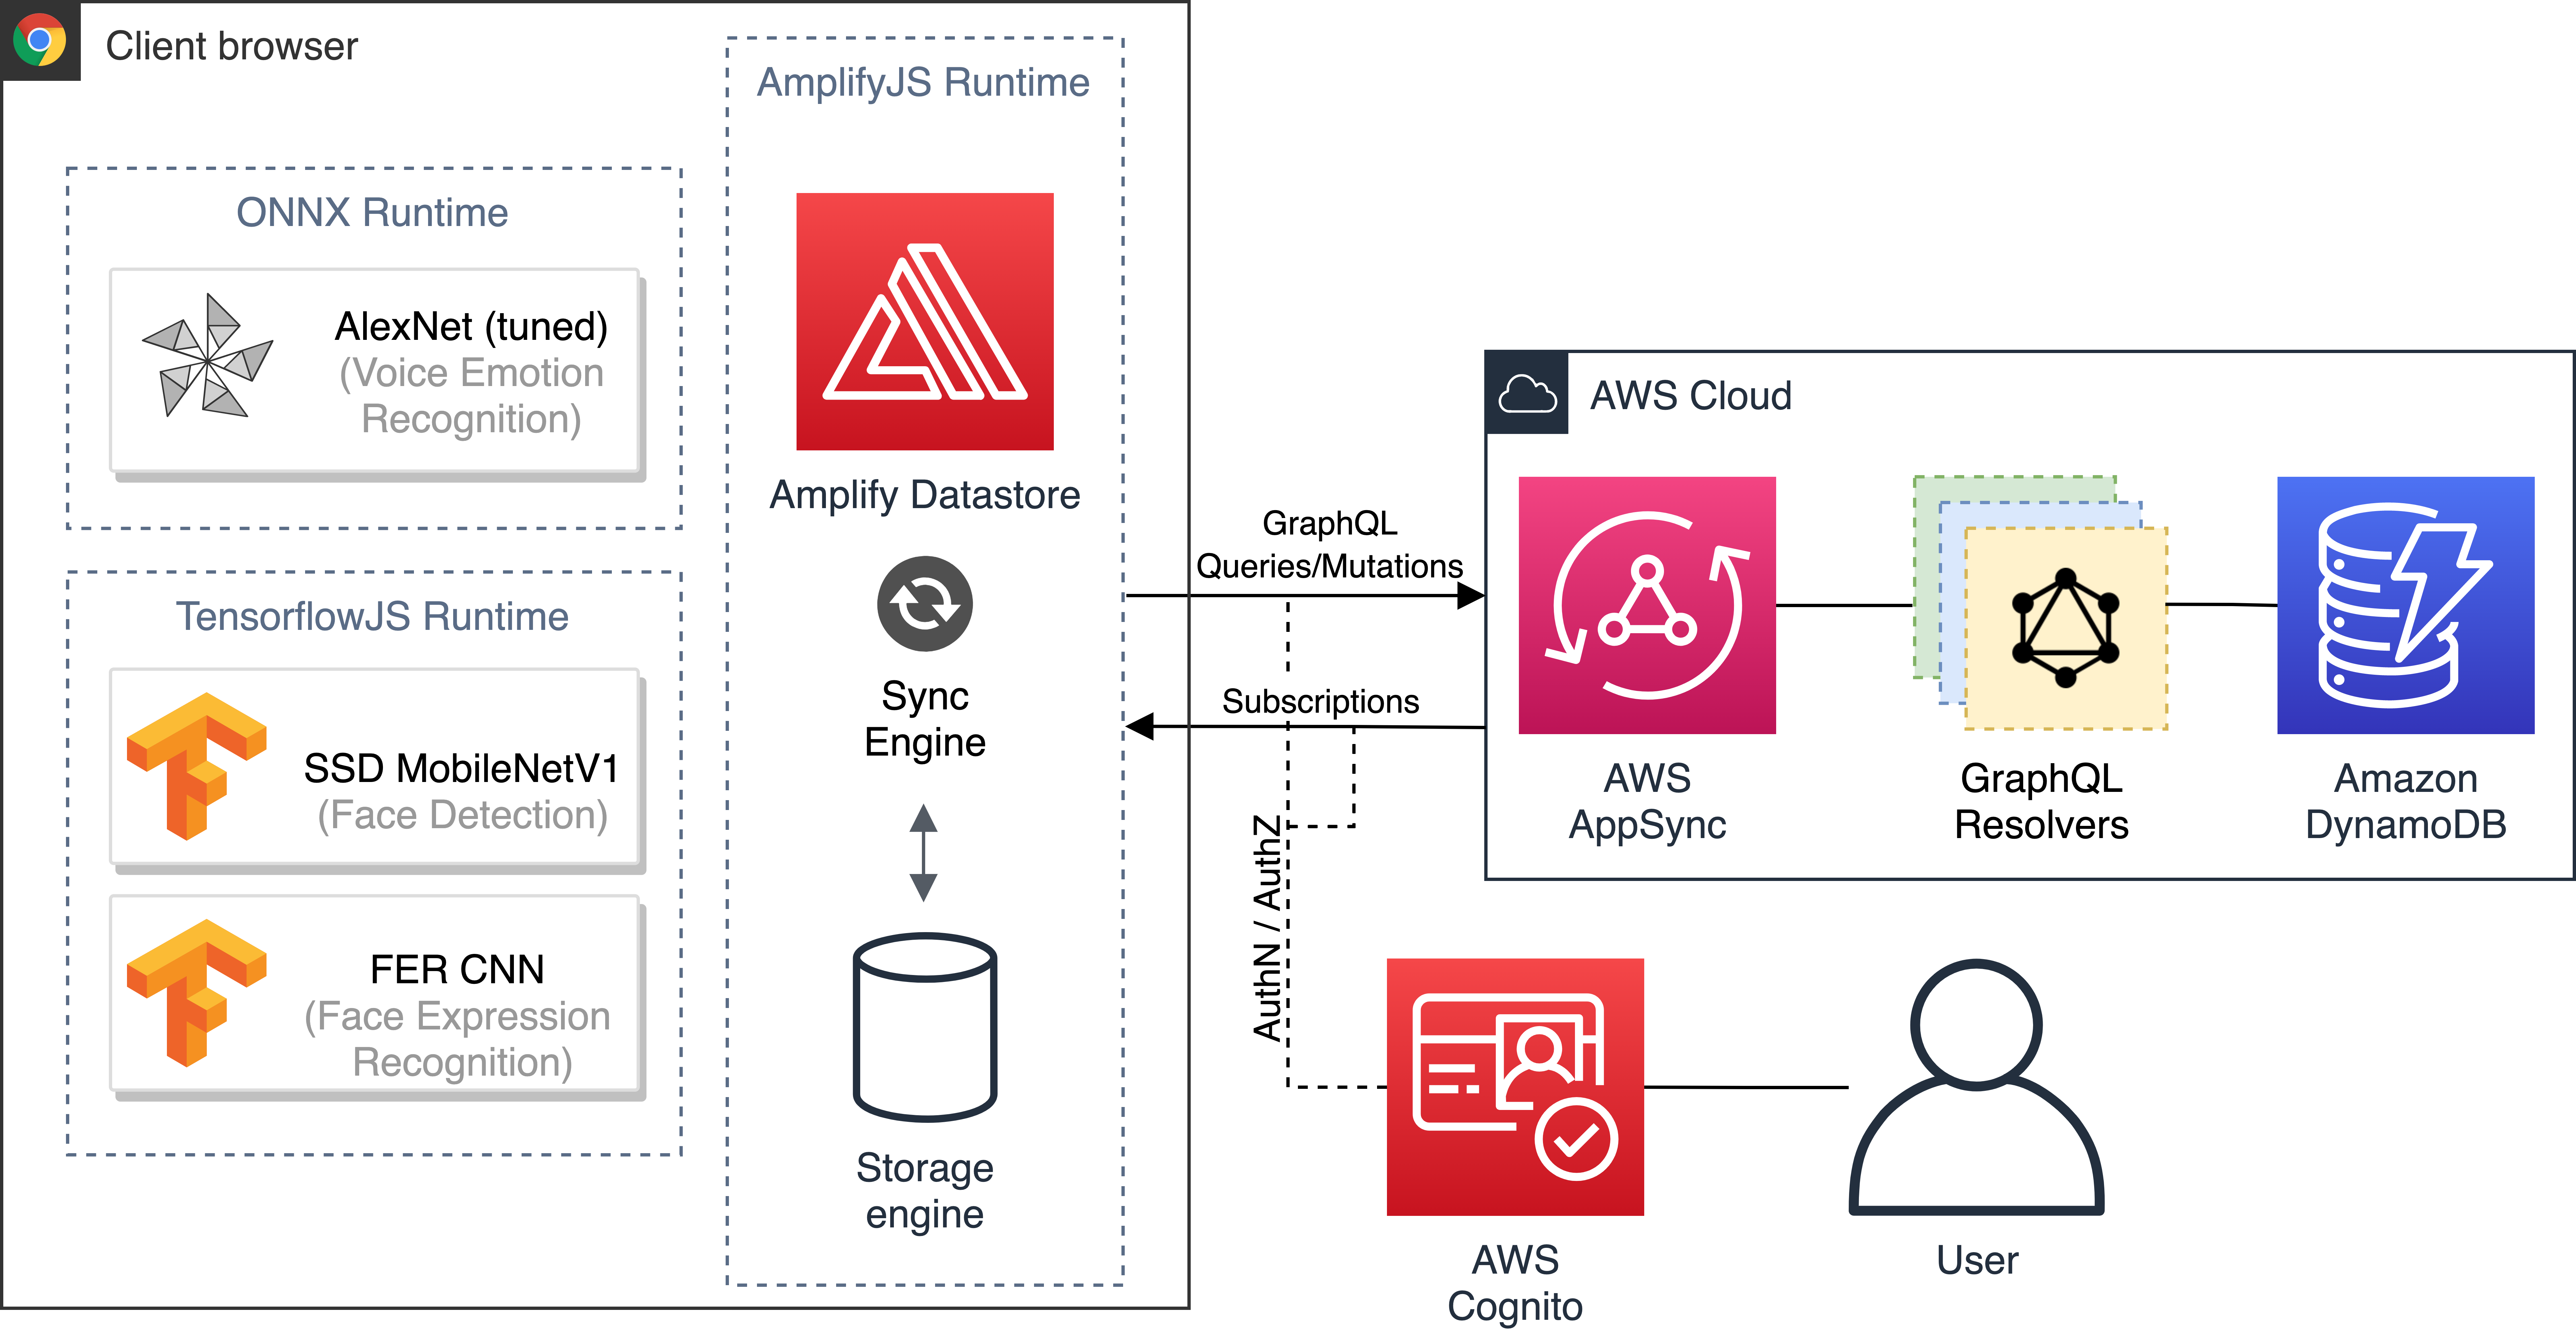
\includegraphics[width=1\textwidth]{assets/system_architecture.png}
\caption{System Architecture Diagram. Moody features a client-server architecture built on top of the AWS platform.}
\label{fig:system_architecture}
\end{figure}

The client-side of the application consists of three major subsystems. The first subsystem is AmplifyJS, which is AWS Amplify's software development kit (SDK) for JavaScript-based applications. For us, it provides the means for data modeling, data persistence across devices as well as user authentication and authorization. Our data is modeled according to the third normal form \cite{codd_further_1972}. The full relational schema can be found in the \nameref{app:appendix}, Figure~\ref{fig:erd}. Amplify Datastore provides an API to a native storage engine that synchronizes asynchronously with the Cloud in the background\footnote{\url{https://docs.amplify.aws/lib/datastore/getting-started/q/platform/js} (last accessed: 07/23/2021)}. The main advantage of this local first approach is a reactive UI because user interaction is decoupled from the network. We keep the UI state consistent across all components using Redux\footnote{\url{https://redux.js.org/} (last accessed: 07/23/2021)} as a state management tool.

The two other subsystems form the machine learning part of Moody. We decided to run all machine learning algorithms locally in the browser of the user. This is beneficial because the internet connection is not impacted by transferring large image and sound data to a remote server every second. In addition, it supports user privacy as only aggregated emotion scores are saved in the Cloud. One drawback is that slower computers might not handle the inference load very well.

The two face models use the TensorflowJS runtime\footnote{\url{https://www.tensorflow.org/js/} (last accessed: 07/23/2021)} and run in a WebGL context\footnote{\url{https://developer.mozilla.org/en-US/docs/Web/API/WebGL_API} (last accessed: 07/23/2021)} allowing for fast computations of the video stream provided by the user. This video stream is captured using the Screen Capture API\footnote{\url{https://developer.mozilla.org/en-US/docs/Web/API/Screen_Capture_API} (last accessed: 07/23/2021)} implemented by all major browsers. As a presenter, you typically want to select the window where the faces of your audience are located. Moody will then detect bounding boxes for these faces and perform expression prediction every second giving the presenter feedback. Please note that at the time of writing it is not possible to select a specific window to share in Safari.

Our voice emotion model is originally written in Python with the PyTorch framework\footnote{\url{https://pytorch.org/} (last access: 07/23/2021)}. As it is not possible to run Python code efficiently in the browser we leverage ONNX. ONNX is a standardized open-source format to represent neural networks as computation graphs and is currently maintained by the community and Microsoft. It comes along with highly optimized runtimes for different platforms with even better inference performance as compared to the original framework (in our case PyTorch) \cite{onnx_runtime_developers_onnx_2021}. \texttt{onnxruntime-web}\footnote{\url{https://github.com/microsoft/onnxruntime/tree/master/js/web} (last accessed: 07/23/2021)} is the browser runtime which we use to run the voice emotion model. Since the WebGL backend is not yet feature-complete we run our model on the client CPU with WebAssembly\footnote{\url{https://webassembly.org/} (last accessed: 07/23/2021)}. WebAssembly is a compilation target for native languages like C(++) or Rust and allows code execution at close to native speed in the browser. It is currently supported by more than 90\% of all browsers\footnote{\url{https://www.tensorflow.org/js/guide/platform_environment#why_wasm} (last accessed: 07/23/2021)}. To capture the sound of the speaker's microphone we utilize the Web Audio API\footnote{\url{https://developer.mozilla.org/en-US/docs/Web/API/Web_Audio_API} (last accessed: 07/23/2021)}. As a speaker, you are also given the possibility to select the input device. When the voice tracking is active Moody will predict voice emotions every 2.1 seconds and give the speaker live feedback.

All data which is collected from user interaction and the machine learning model predictions is persisted in the AWS Cloud to be available across devices and for further research analysis. Therefore, we have deployed a GraphQL API endpoint with AWS AppSync\footnote{\url{https://aws.amazon.com/appsync/} (last accessed: 07/23/2021)}. This endpoint is called by Amplify Datastore in the background to synchronize new data with the backend. AppSync authorizes each request with AWS Cognito which we use for user authentication. As AppSync is data source agnostic it needs resolvers telling it how to interact with a backend. We chose DynamoDB as the database backend\footnote{\url{https://aws.amazon.com/dynamodb/} (last accessed: 07/23/2021)}. Luckily, Amplify creates these resolvers automatically given a GraphQL compliant data schema\footnote{\url{https://spec.graphql.org/June2018/#sec-Type-System} (last accessed: 07/23/2021)}.

\subsection{Facial Emotion Recognition}
\label{subsec:method_facial_emotion_recognition}
We implement our facial emotion recognition with the \texttt{faceapi.js}\footnote{\url{https://justadudewhohacks.github.io/face-api.js/docs/index.html} (last accessed: 07/23/2021)} JavaScript API for face detection, which is implemented itself on top of the TensorFlowJS core API and can perform face recognition in the browser. To execute in this project both, the face detection itself and the face expression/emotion recognition, we use two neural networks. The input data are single images from the live video conference, which are picked up from the meeting tool (e.g. Zoom) window where the participants' cameras appear. This desktop window has to be selected by the Moody user before he starts the emotion tracking. The two models, which are briefly presented below, were already developed and provided by the authors of \texttt{faceapi.js}, which is why no more data preprocessing was necessary and these only had to be implemented in our system architecture.

First, the algorithm has to detect the faces in the live video and create bounding boxes around the corner points of the faces. For this purpose \texttt{face-api.js} uses the SSD (Single Shot Multibox Detector) MobileNetV1 face detection model\footnote{\url{https://justadudewhohacks.github.io/face-api.js/docs/classes/ssdmobilenetv1.html} (last accessed: 07/30/2021)} \cite{howard_mobilenets_2017}. The neural net will compute the positions of each face in a picture and return the bounding boxes and their occurrence probabilities for each face. Instead of then focusing on short inference time, this face detector aims for high accuracy in recognizing face bounding boxes. Nevertheless, the size of the quantized model is rather small at about 5.4 MB and thus it works at an acceptable speed. This face detection model has been trained on a dataset called 
\emph{WIDERFACE} which was developed by the authors \citeA{yang_wider_2016} and is a face detection benchmark dataset from publicly available images. The authors chose 32,303 images and labeled 393,703 faces on these with a high degree of variability in scale, pose, and occlusion. The weights for the SSD MobileNetV1 model and the final face detector, powered by the TensorFlow object detection API\footnote{\url{https://github.com/tensorflow/models/tree/master/research/object_detection} (last accessed: 07/30/2021)} and trained by \citeA{yang_wider_2016}, were provided by yeephycho\footnote{\url{https://github.com/yeephycho} (last accessed: 07/23/2021)} in a GitHub-Repository\footnote{\url{https://github.com/yeephycho/tensorflow-face-detection} (last accessed: 07/23/2021)}.

The second neural net uses the detected faces and their bounding boxes as an input for the facial expression recognition model. When all faces were detected on an image, the model receives this information and returns an array consisting of all detected faces and their belonging face expressions. The input images in our tool are single frozen frames of the videoconference camera screen. The authors of \texttt{faceapi.js} claim that it is fast and provides reasonable accuracy. The model is about 310 kB in size and uses depthwise separable convolutions as well as densely connected blocks. It was trained on a variety of photos, including photographs scraped from the web and images from publicly available sources. Wearing glasses or low light conditions may reduce the accuracy of the prediction results.

\subsection{Vocal Emotion Recognition}
\label{subsec:method_vocal_emotion_recognition}
In the following sections, we will explain how we preprocess our data regarding our voice emotion model, as well as how we set the model up and train it. We use the datasets introduced in Section~\ref{sec:related_work} as well as a self-designed CNN based on an AlexNet architecture.

\subsubsection{Data Preprocessing}
\label{subsubsec:method_vocal_emotion_recognition_data_preprocessing}
The input we will need later for our voice model is the waveform of the sound which needs to be preprocessed. To avoid fitting the dataset specific volume of the audio samples we apply RMS audio normalization. It is a form of loudness normalization which brings heterogeneous audio sequences to a consistent sound level. We use the formula described by Equation \ref{eq:rms_normalization} for this purpose where $y_n$ is the $n^{th}$ normalized audio sample and $x_n$ the original audio sample in an audio sequence of $N$ samples in total. $r$ is a hyperparameter describing the target RMS level\footnote{\url{https://pydiogment.readthedocs.io/en/latest/_modules/pydiogment/auga.html#normalize} (last accessed: 07/23/2021)}:
\begin{equation}
\label{eq:rms_normalization}
y_n=\sqrt{\frac{N-10\,(\frac{r}{20})}{\sum_{i=0}^{N-1}{x_i^2}}}\cdot{}x_n
\end{equation}
Then the normalized waveform is converted into Mel spectrograms. This step is part of a feature extractor block in the final neural network. We use 128 Mel coefficients. We do this with the \texttt{torchlibrosa} library \cite{kong_panns_2020}. In this library we have re-implemented the Short-Time-Fourier-Transform (STFT) as a CNN with Conv2d layers so that it is compatible with \texttt{onnxruntime-web} \cite{onnx_runtime_developers_onnx_2021}. The STFT is a Fourier Transform version that uses a sliding time window to break up the audio signal into smaller chunks. We use a window size of 2,048 and a sample rate of 22,050. It takes each section of the Fast Fourier Transform (FFT) and then combines them. As a result, it can catch changes in frequency over time \cite{griffin_signal_1984}. To get in the end more data and therefore better training results, we augmented our existing data sets (RAVDESS, TESS, JL-Corpus, EMO-DB) with common data augmentation methods. We used stretching and squeezing (randomly slow down or speed up the sound), background noise (add some random values to the sound), random shifting (shift audio to the left or the right by a random amount), left- and right-trimming (cut off any silence in the beginning or end), and pitch tuning (randomly modify the frequency of parts of the sound)\cite{mcfee_librosa_2015}. The voice emotions are recorded in time windows of 2.1 seconds. This time is the average duration of the samples in the datasets we use.

\subsubsection{AlexNet Architecture}
\label{subsubsec:method_vocal_emotion_recognition_alexnet_architecture}
The input for the voice emotion model is an RMS-normalized sound sequence of length 463,050. In a first feature extractor block, the neural network automatically extracts Mel spectrograms from the sound waveform as described in Section~\ref{subsubsec:method_vocal_emotion_recognition_data_preprocessing}. A major advantage of having the feature extraction as part of the model is that this step does not have to be re-implemented for each programming language -- in our case JavaScript -- thus leading to consistent preprocessing and prediction results independent of the environment.

These Mel spectrograms serve as input for the convolutional neural network part. Based on the datasets introduced in Section~\ref{subsec:related_work_vocal_emotion_recognition} we train the model. We have tried out two well-known architectures: ResNet18 and AlexNet \cite{krizhevsky_imagenet_2012,he_deep_2015}. The performance of both models is very similar, only the size of the models differs. Since the AlexNet with 32.3 MB is almost half the size of the ResNet18 with 59.7 MB and has fewer parameters, we decided to use the AlexNet for our web app (cf. Section~\ref{subsec:results_vocal_emotion_recognition}). This is then exported to ONNX to be executed in the browser with the help of \texttt{onnxruntime-web} for inference.

Additionally, we have modified the default AlexNet architecture with the goal to reduce overfitting by adding batch normalization, layer normalization, and dropout layers. Figure~\ref{fig:alexnet_architecture} illustrates the detailed architecture. Since we use cross-entropy loss\footnote{\url{https://pytorch.org/docs/stable/generated/torch.nn.CrossEntropyLoss.html} (last accessed: 08/02/2021)} as loss function the model output are the raw logits. Applying the softmax function\footnote{\url{https://pytorch.org/docs/stable/generated/torch.nn.functional.softmax.html} (last accessed: 02/08/2021)} on this vector will yield the corresponding class probabilities for each emotion.

\begin{figure}
    \centering
    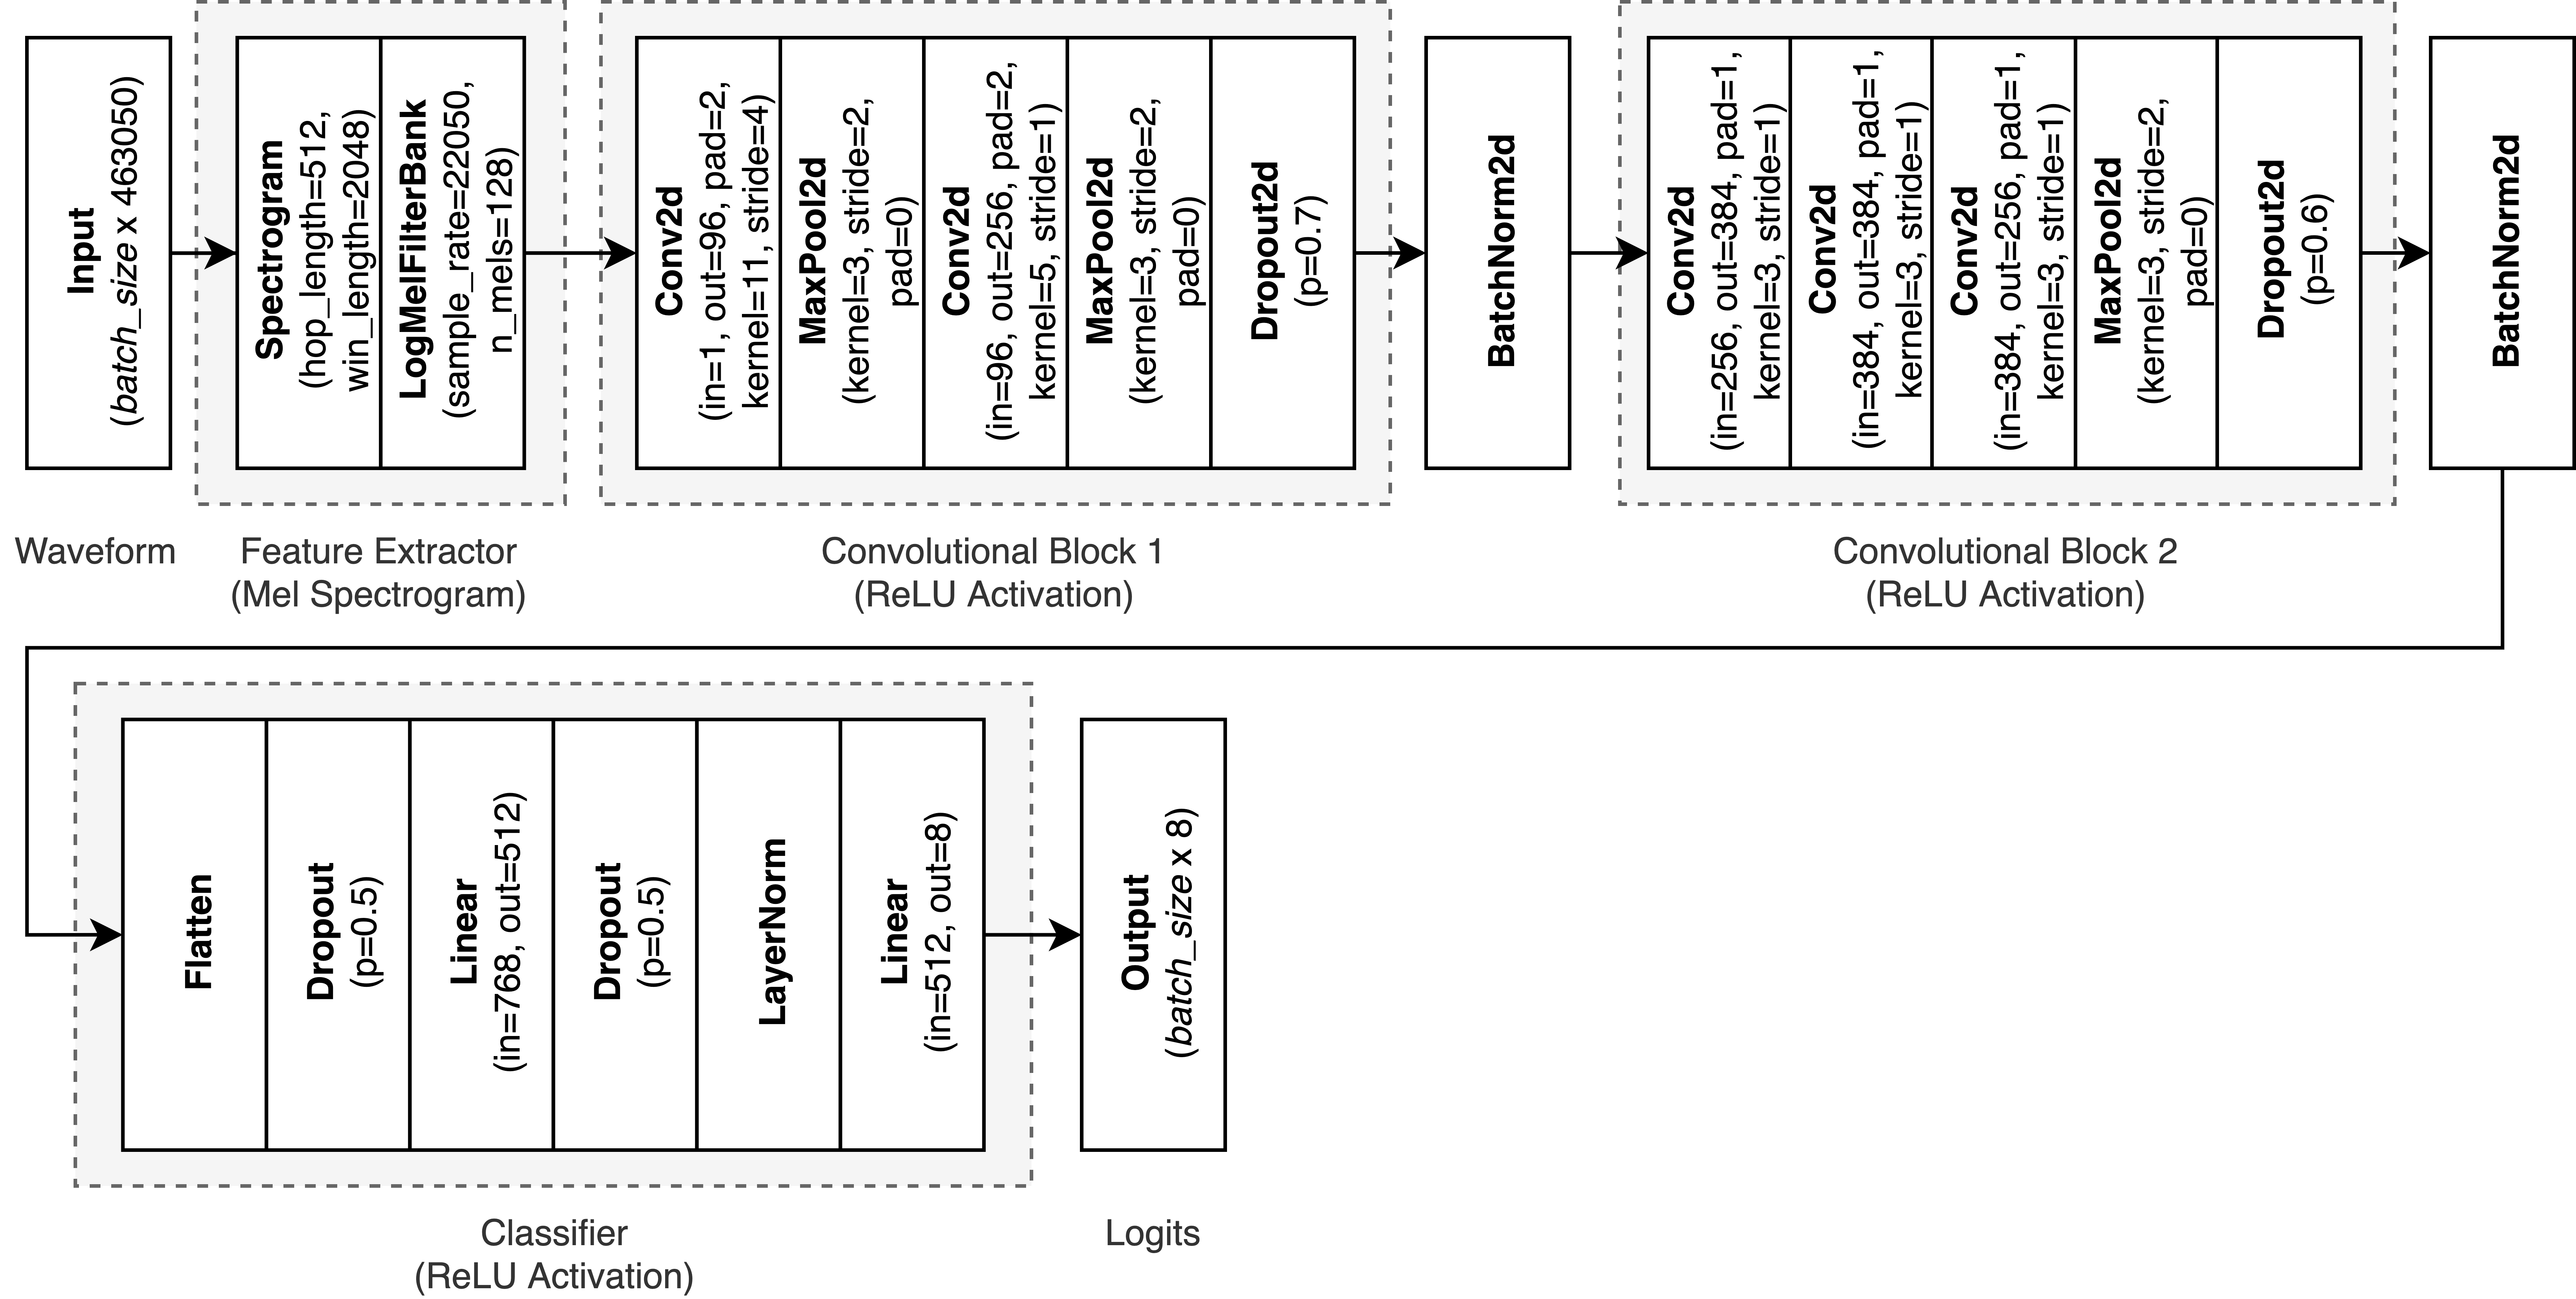
\includegraphics[width=\textwidth]{assets/alexnet_architecture.png}
    \caption{The modified AlexNet architecture of Moody's voice emotion model. All \emph{Conv2d} and \emph{Linear} layers are connected via the ReLU activation function.}
    \label{fig:alexnet_architecture}
\end{figure}

\section{Results}
\label{sec:results}
In this section, we show the outcomes of the implemented system architecture as well as the facial and vocal emotion recognition as described in Section~\ref{sec:method}.

\subsection{Experiment Environment \& Testing Setup}
\label{subsec:results_experiment_environment_and_testing_setup}
We conducted our experiments during a virtual seminar ``Collaborative Innovation Networks'' (COINs) in the summer semester of 2021 held by Prof. Peter Gloor (MIT). The seminar consisted of 23 students from the Universities of Cologne, Bamberg and Lucerne and three instructors. All students formed in total six teams with three to five participants working on complex subject-related and practical topics. Due to the global COVID-19 pandemic at that time and agile project management, all teams presented their results in weekly and bi-weekly sprints during a virtual Zoom meeting. In these virtual status meetings, every group presented their project goals, progress, results or plans of the last and next iteration and a retrospective in a short presentation of approximately ten minutes.

Since our prototype Moody was not ready for use right at the first meeting and still needed to be developed to track emotions we were only able to ask the other groups to use our Moody Tracker from the third meeting onwards. For this purpose, we wrote a short usage guide within the invitation before the meeting, so that each group could activate the tracker during their presentation. Therefore, in addition to the usage instructions, we asked the other teams to generate a feedback link via our website (\url{www.moody.digital}) after their presentation and share it with the other meeting participants.

The underlying intention here was primarily to receive instant feedback about our application in real-world usage. This made continuous testing possible, which enabled us to constantly work on errors and bugs reported by the users in each status meeting. Also, we had the chance to quickly collect subjective ratings about the perceived quality of each presentation and compare it to the tracked emotion data. The focus of this paper lies neither in statistically analyzing the correlation nor the causality between the experienced emotionality of the audience and the presentation quality, but we had the chance to cursorily analyze the first insights.

Exemplarily, Figure \ref{fig:moody_statistics_screenshot} shows a screenshot of the recorded statistics of our status presentation on the 6th July 2021. With this recording, we found that our last presenter on that day seemed to speak rather sad than happy. He was able to use this information for the next presentation to increase his positive emotion transmissions via voice. Additionally, we have seen that the faces and voices were interpreted mainly neutrally, because of the formal and informative character of the presentations. This aligns with our expectations and indicates that the models are predicting correctly.

\begin{figure}
\centering
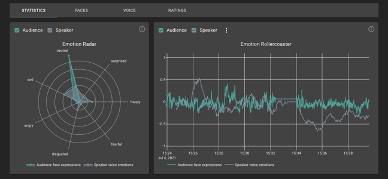
\includegraphics[width=1\textwidth]{assets/moody_statistics_screenshot.png}
\caption{Caption}
\label{fig:moody_statistics_screenshot}
\end{figure}

\subsection{Face Emotion Recognition}
\label{subsec:results_face_emotion_recognition}
Since we adopt the pre-developed \texttt{faceapi.js} and its two underlying models for face detection and expression recognition, we do not want to focus in this chapter on presenting the resulting metrics and accuracies. Instead, we briefly show that we implemented the API correctly in our tool and how it works. Figure \ref{fig:moody_faces_screenshot} illustrates the presenter's view of the detected faces and their current emotions when he clicks on the Tab ``Faces'' while the emotion tracking is running. It seems that the model identifies the emotionalities expressed by the faces correctly.

\begin{figure}
\centering
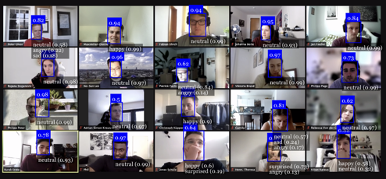
\includegraphics[width=1\textwidth]{assets/moody_faces_screenshot.png}
\caption{Caption}
\label{fig:moody_faces_screenshot}
\end{figure}

The models receive every second a freeze frame from the video conference window with all participants' cameras and calculate every second the probabilities for the current face emotion per person respectively per detected face. The probabilities are shown as values between 0 and 1. Exemplarily, ``happy (0.8)'' and ``neutral (0.2)'' mean that the particular face looks like 80\% happy and smiling and 20\% neutral. paul ekman emotions...
 if a face 99\% smiles and looks happy. Every emotion from. The formula 
formel:
\begin{itemize}
\item score zusammensetzung: https://github.com/COINS-SS21/moody/blob/main/src/meetings/speakerVoiceEmotionUtils.ts, der score ist pro person und dann noch der durchscnitt von allen teilnehemern
\end{itemize}

\subsection{Vocal Emotion Recognition}
\label{subsec:results_vocal_emotion_recognition}
Since the AlexNet was trained on the four different sets of data (RAVEDESS, EMO-DB, TESS, JL-Corpus) to get as much variety as possible, the accuracy of the model was about 87.17\% (cf. Figure \ref{fig:alexnet_accuracy}). 

\begin{figure}
\centering
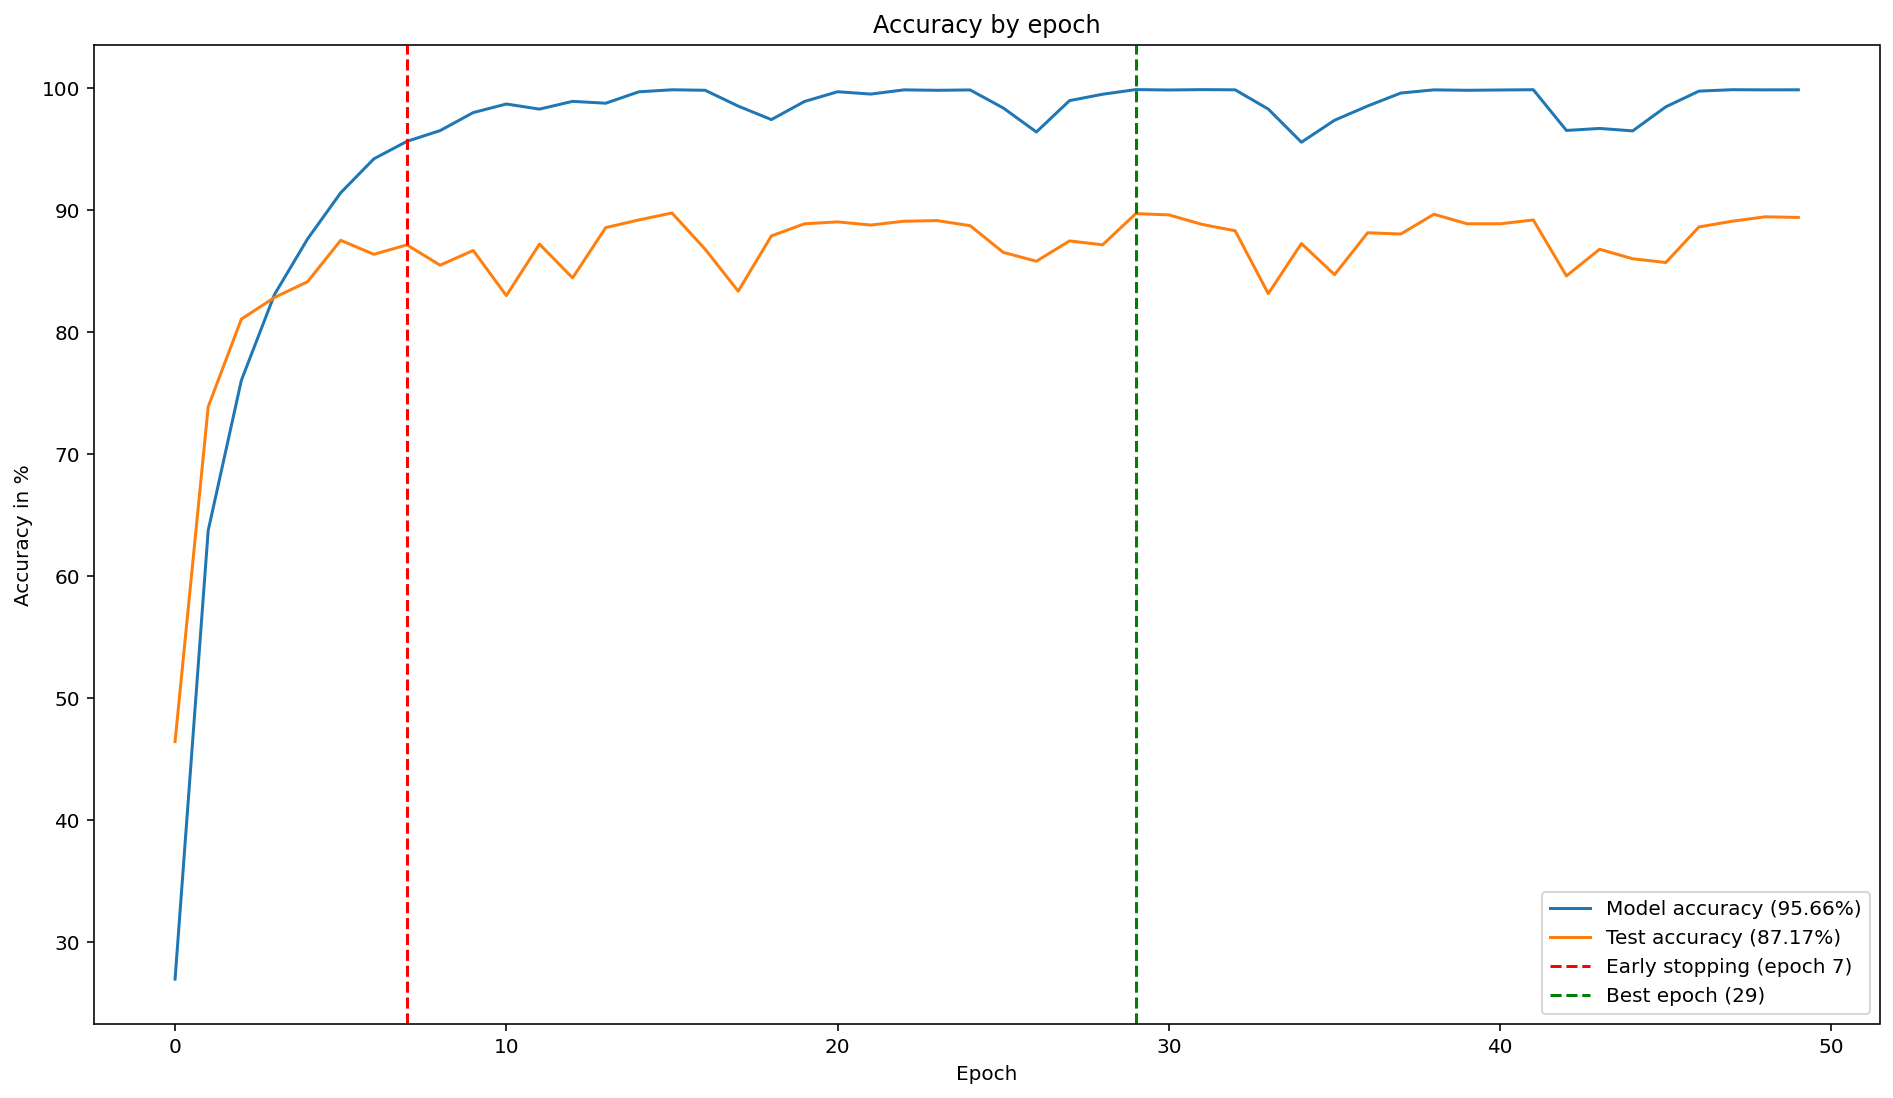
\includegraphics[width=1\textwidth]{assets/alexnet_accuracy.png}
\caption{Accuracy by Epoch}
\label{fig:alexnet_accuracy}
\end{figure}

To get the best possible result, early stopping was included. This was best at the eighth epoch, as the loss did not change much there either (cf. Figure \ref{fig:alexnet_loss}).

\begin{figure}
\centering
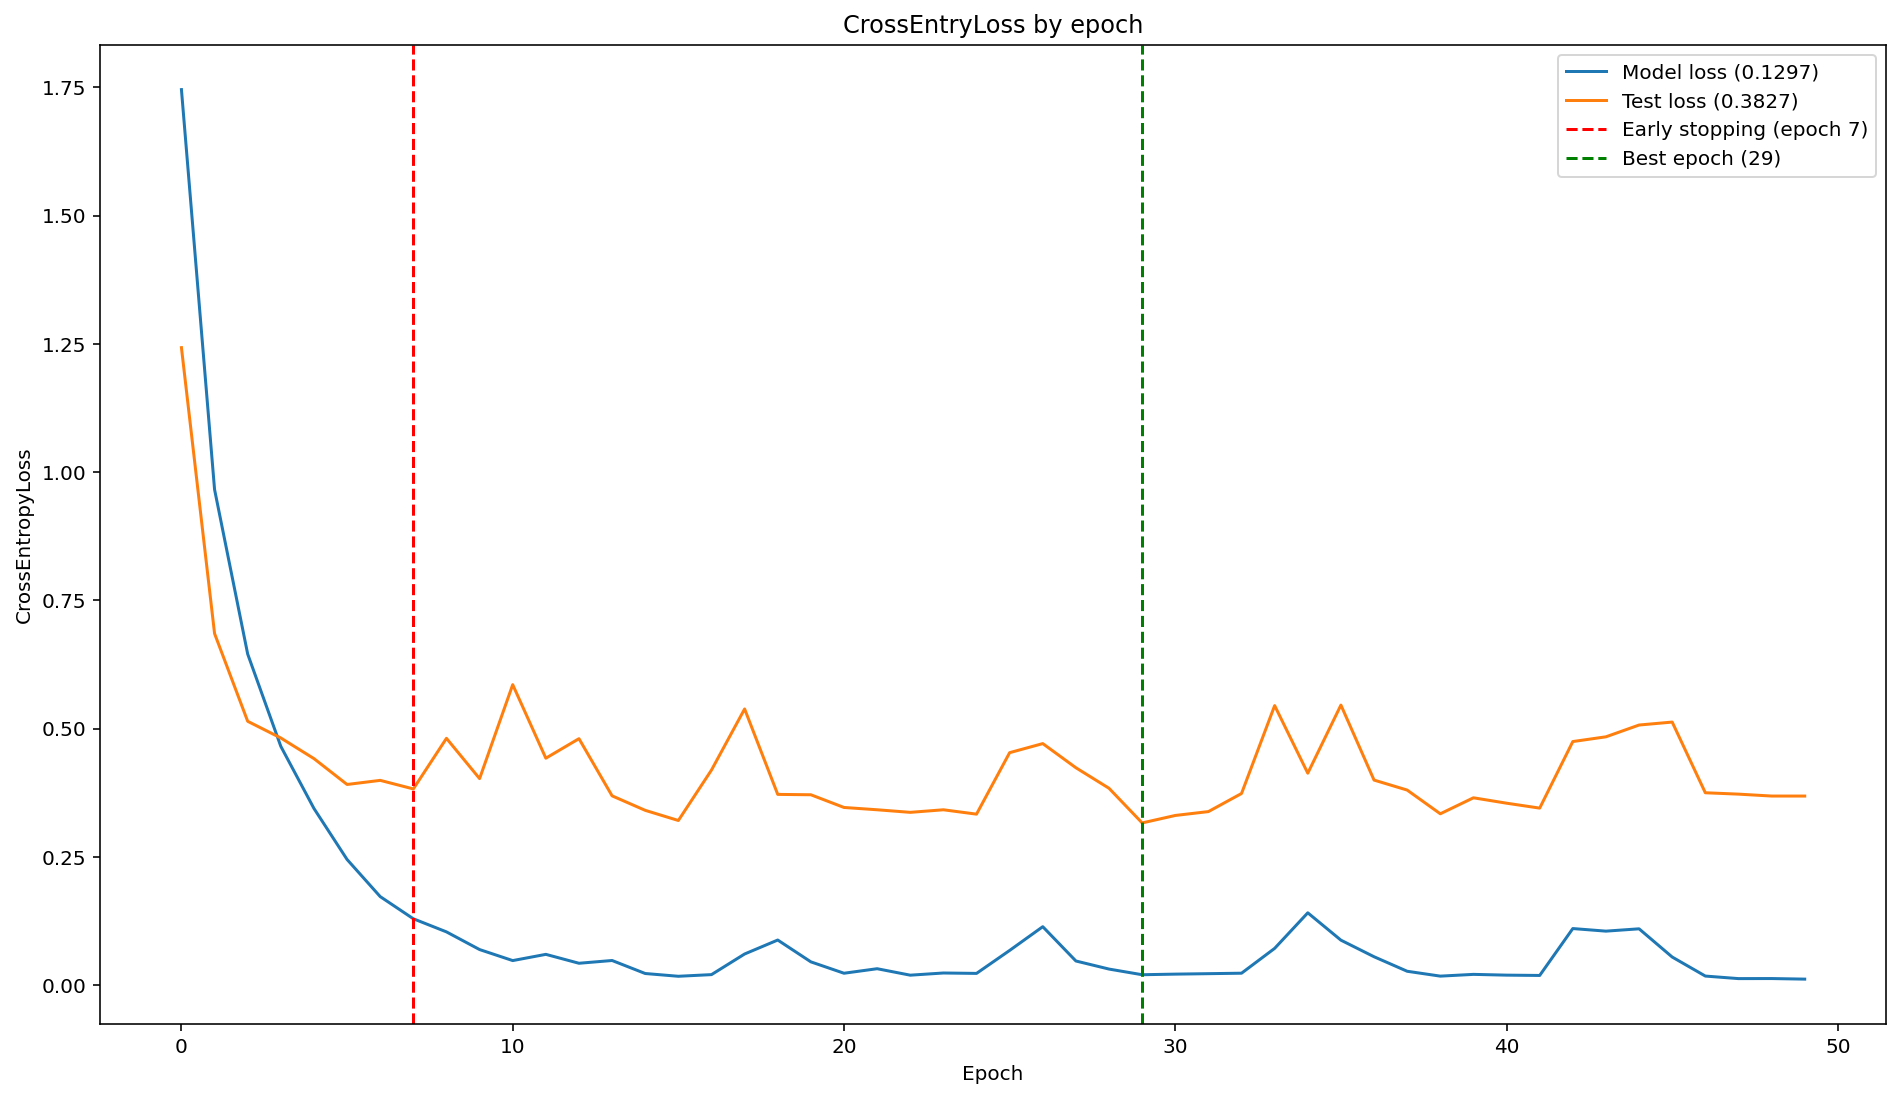
\includegraphics[width=1\textwidth]{assets/alexnet_loss.png}
\caption{Cross Entry Loss by Epoch}
\label{fig:alexnet_loss}
\end{figure}

The difference to the ResNet model, apart from minor differences in accuracy, was mainly the size of the model. The AlexNet has a size of 32.3 MB whereas the ResNet is almost twice as big with a size of 59.6 MB. Since the data model is reloaded in the browser every time the voice emotion model is used, which takes up time as well as memory, we finally decided to use the AlexNet. It has solid accuracy and smaller memory size which is ideal for usage on end-user devices.

\begin{figure}
\centering
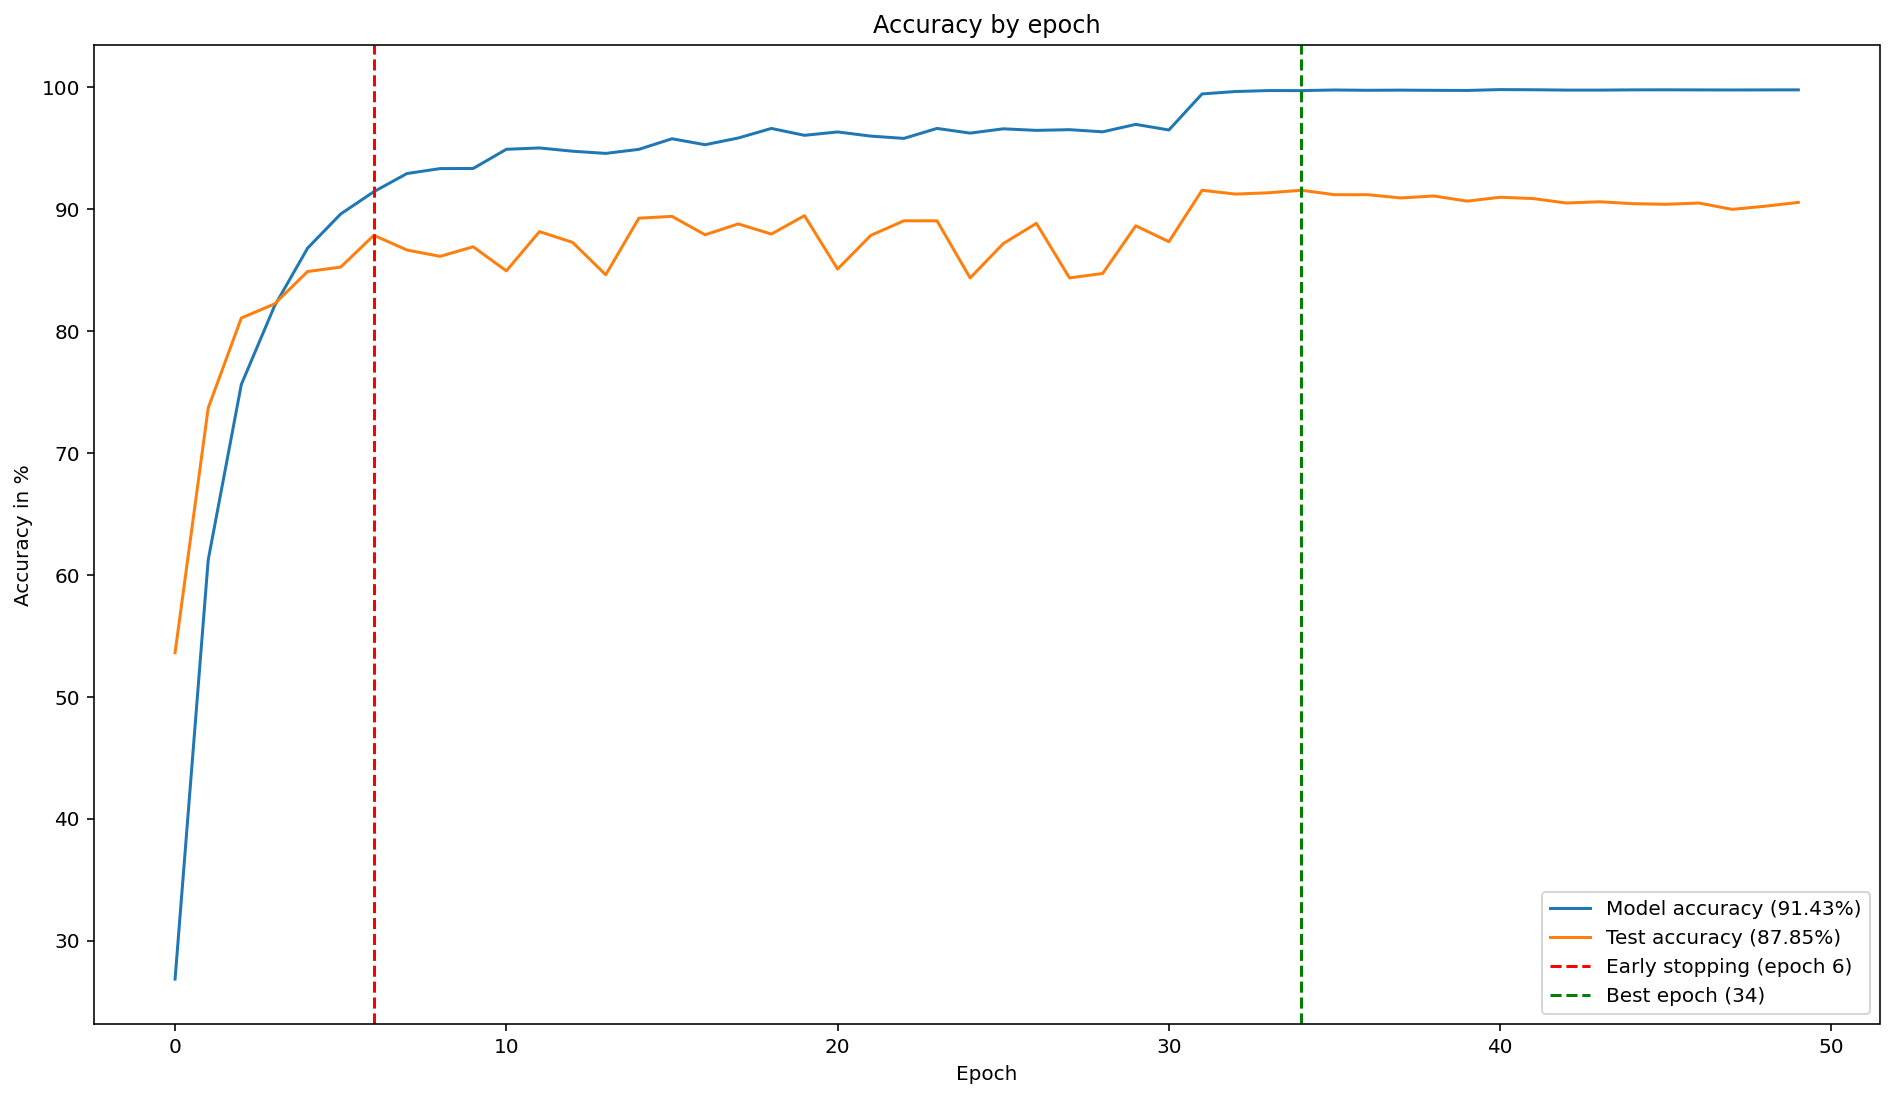
\includegraphics[width=1\textwidth]{assets/resnet_accuracy.png}
\caption{ResNet Accuracy}
\label{fig:resnet_accuracy}
\end{figure}

Finally, the confusion matrix shows that our model has fairly high prediction values and very low deviations for all emotions (cf. Figure \ref{fig:alexnet_confusion_matrix}).

\begin{figure}
\centering
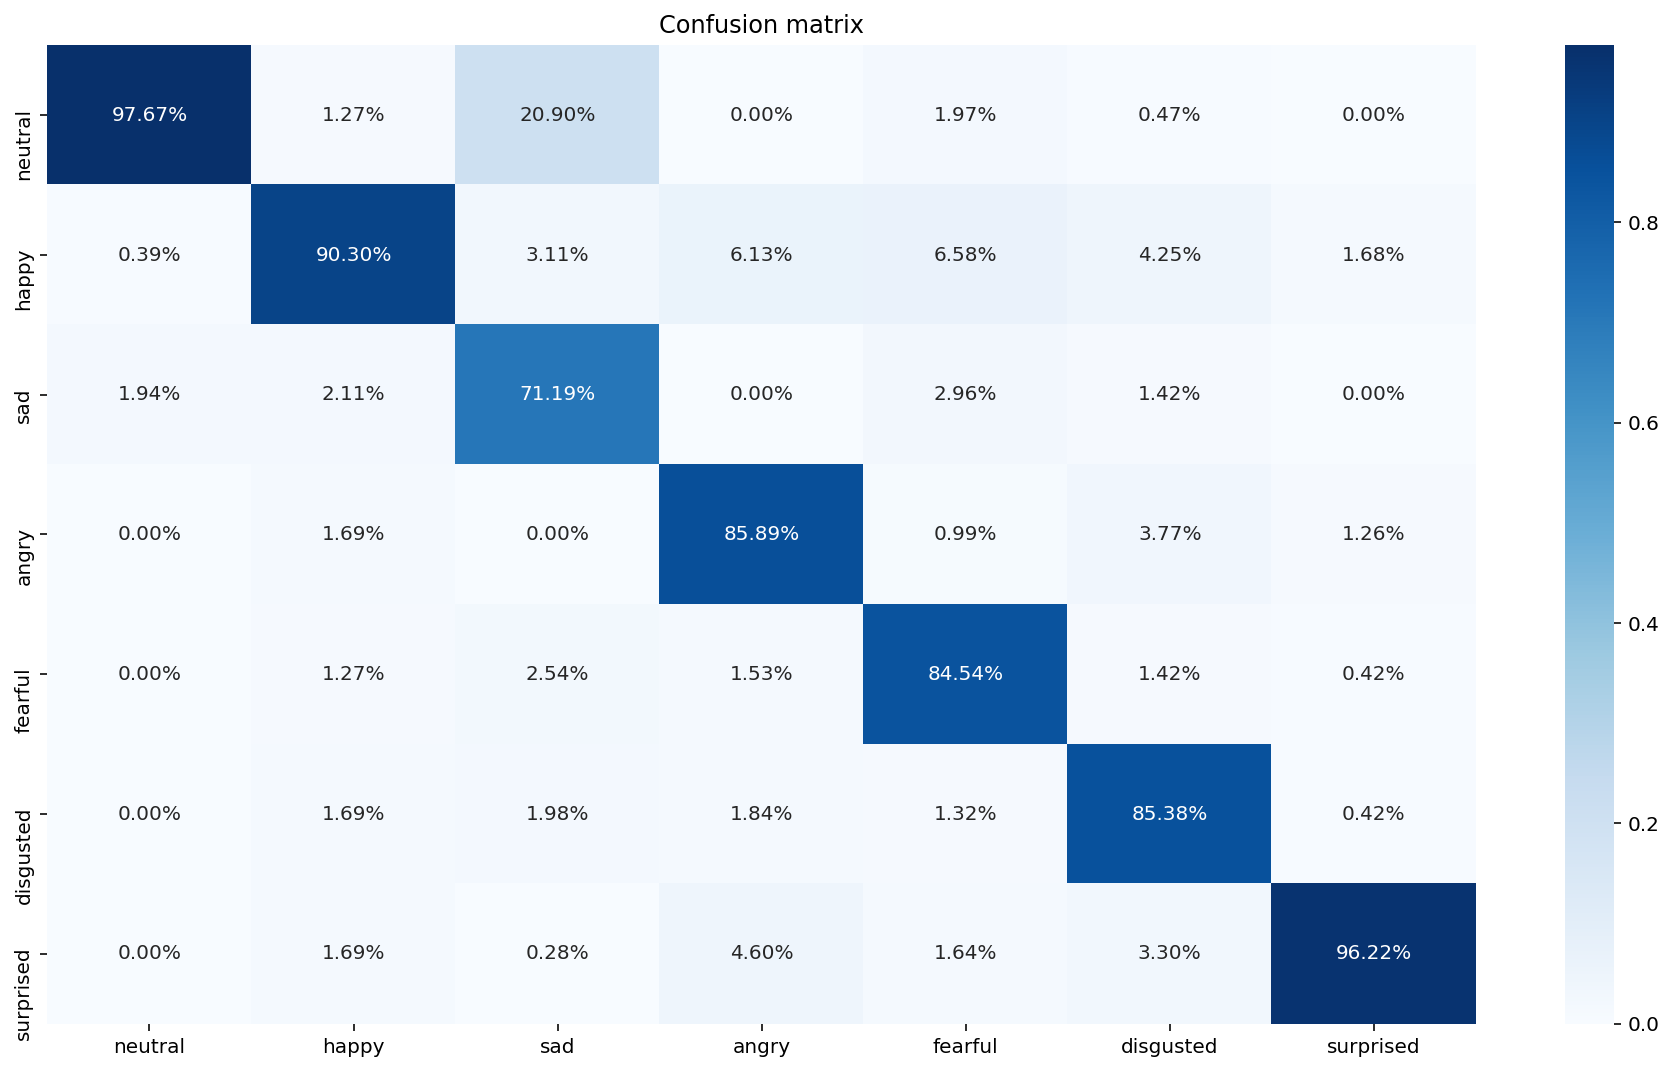
\includegraphics[width=1\textwidth]{assets/alexnet_confusion_matrix.png}
\caption{AlexNet Confusion Matrix}
\label{fig:alexnet_confusion_matrix}
\end{figure}

The voice emotion model can be activated optionally at any time during a meeting. It can be added during any meeting or just at the beginning of the meeting and will be then downloaded through the browser. During the meeting, in addition to the emotion roller-coaster, the voice emotions can also be determined at the current time. A time span of 2.1 seconds is always taken to track the current emotion, which is delivering a good prediction of the emotion at that moment. At the end of the meeting a moving average can be calculated, looking at all the voice emotion tracked in that meeting, to get the most valuable and usable result.  

\section{Discussion}
\label{sec:Discussion}
In this seminar paper we describe how we built our moody.digital web application, and how it recognises face emotion with the face.api, and voice emotion with our self-built AlexNet. The web app is an extension of the existing web app from the previous semester of the COINs seminar at the University of Cologne in collaboration with the University of Bamberg and the University of Applied Science and Arts in Lucerne. The previous project already built an application that was able to track the face emotion live during virtual meetings. With our additions, the app has gained further features. For one thing, it is now able to recognise live voice emotion in addition to face emotion. Both emotions are displayed live during the meeting in an emotion roller-coaster. In addition to the live components, the data is also stored in the database for post analysis. In this way, you can look at all the emotions of the meetings that have already been completed and evaluate them as you wish. The feedback from the audience can also be viewed and analysed.In our Zoom meetings during the COINs seminars, we were able to determine the first correlation between the face and the voice emotions (cf. Figure \ref{fig:moody_statistics_screenshot}). In order to draw a meaningful conclusion, further video meetings must be analysed with the tool. However, based on the accuracy of the emotion recognition models, we have designed an app that recognises these with a high accuracy and is therefore capable of such analyses. 
With this application we have built a tool, with which future presenters can improve their style of presentation and get more audience with it. It can also be used for further research purposes to gain more insights about presentations.

\section{Limitations and Future Work}
\label{sec:limitations_and_future_work}
While the Moody web app is able to capture and persist emotions with reasonable accuracy in real-time during virtual meetings, there is still potential for improvement and future work. In addition, at the time of writing, certain limitations are imposed by the early stage of development of \texttt{onnxruntime-web} and the implementations of web standards in major browsers.

The current implementation of the voice emotion model predicts the speaker's vocal emotions in windows of 2.1 seconds. This way of predicting is unfortunately prone to the start and end of a sound sequence even though we already counteract this behavior by using random shifting during data augmentation. One way to make the model more robust against shifted sentences might be the usage of a rolling estimator. Instead of predicting in 2.1-second windows, one could add three estimators each shifted by 0.3 seconds and perform three additional predictions on the shifted sound sequences. In the end, one would reconcile the results to one predicted value, for example by averaging. This way, the impact on the prediction result of sentences starting in one window and ending in another window can eventually be reduced.

A limitation going in line with the rolling estimator is the computational power required to perform multiple predictions simultaneously. As the machine learning model runs on the end-user device it is important not to impact the user experience. \texttt{onnxruntime-web} does not yet support all operators needed by the voice model in WebGL\footnote{Current status can be checked here: \url{https://github.com/microsoft/onnxruntime/tree/master/js/web#webgl-backend} (last accessed: 07/29/2021)}. Therefore, it might be necessary to wait until the GPU-accelerated WebGL context is supported by ONNX before implementing this feature.

Another hypothesis for improving the voice emotion recognition accuracy is to add more data (e.g. by creating an own dataset) and to try out language and gender-specific models.

A limitation of the current web app is the feature completeness of Web Media APIs in different browsers. For example, Safari does not allow selecting a specific window when sharing the user screen. This way it is not possible to use the Moody app with only one screen. Mozilla Firefox does not support an audio sample rate different from the default sample rate of the user device\footnote{Current status can be checked here: \url{https://developer.mozilla.org/en-US/docs/Web/API/MediaTrackConstraints/sampleRate} (last accessed: 07/29/2021)}. This leads to some users not being able to use the voice emotion recognition if their device does not use the sample rate 22,050 which the model expects.


\newpage
\section*{Appendix: Relational Data Model}
\label{app:appendix_relational_data_model}
\begin{figure}[ht]
\label{fig:erd}
\centering
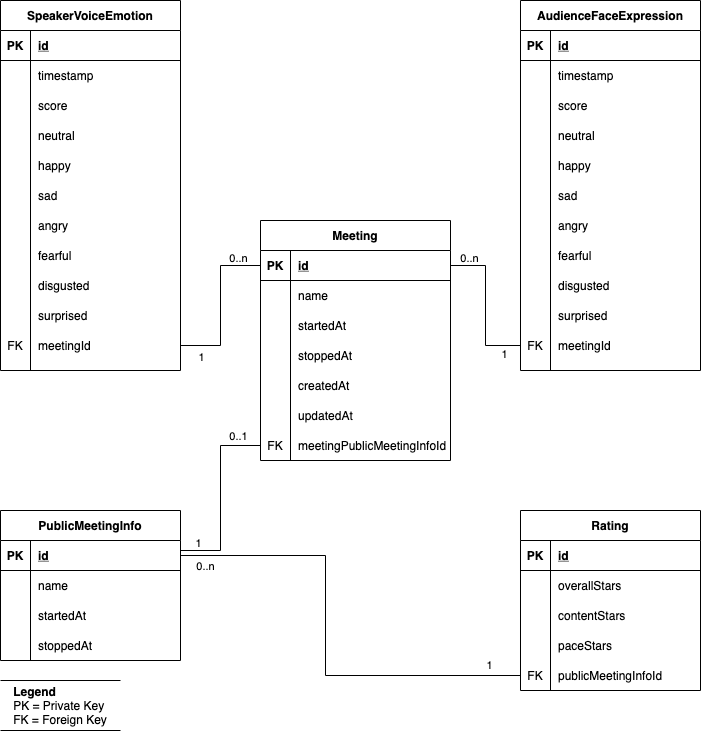
\includegraphics[width=1\textwidth]{assets/erd.png}
\caption{The entity relationship diagram (ERD) for the database structure of Moody. Relationships are modeled in UML style. Each table has an additional owner field  storing the user id from AWS Cognito which is omitted in the illustration for brevity.}
\end{figure}

\newpage
\printbibliography
\end{document}
